% !TEX program = xelatex
% !TEX encoding = UTF-8 Unicode
% !TEX spellcheck = de_US

% --------------------------------------------------------------------------- %
% Poster template for Institute of Telematics.      						  %
% --------------------------------------------------------------------------- %
% Created with Brian Amberg's LaTeX Poster Template. Please refer for the     %
% attached README.md file for the details how to compile.				      %
% --------------------------------------------------------------------------- %
% $LastChangedDate:: 2017-08-03 18:00:00 +0200 (V, 12 szept. 2017)          $ %
% $LastChangedRevision:: 129                                                $ %
% $LastChangedBy:: allner                                                   $ %
% $Id:: poster.tex 128 2011-09-11 08:57:12Z rlegendi                        $ %
% --------------------------------------------------------------------------- %


\documentclass[a0paper,portrait]{baposter}

\usepackage[utf8]{inputenc}
\usepackage{relsize}		% For \smaller
\usepackage{url}			% For \url
\usepackage{epstopdf}	% Included EPS files automatically converted to PDF to include with pdflatex
\usepackage{verbatimbox}
\usepackage{enumitem}
\usepackage{wrapfig}
\usepackage{natbib}
\usepackage{setspace}
\usepackage{uzlcolor}
\usepackage[english]{babel}
\usepackage{blindtext}
\usepackage{amsmath} 



%%% Myriad Pro Font - %%%%%%%%%%%%%%%%%%%%%%%%%%%%%%%%%%%%%%%%%%%%%%%%%%%%%%%%%
\usepackage{fontspec}
\defaultfontfeatures{Mapping=tex-text,Scale=MatchLowercase}
\setmonofont{Myriad Pro}
\setmainfont[
BoldFont={Myriad Pro}, 
ItalicFont={Myriad Pro},
BoldItalicFont={Myriad Pro}
]{Myriad Pro}
\setsansfont{Myriad Pro}



%%% Global Settings %%%%%%%%%%%%%%%%%%%%%%%%%%%%%%%%%%%%%%%%%%%%%%%%%%%%%%%%%%%
\graphicspath{{pix/}}	% Root directory of the pictures 
\tracingstats=2			% Enabled LaTeX logging with conditionals

\newcommand{\localtextbulletone}{\textcolor{uzl_orange_2}{\raisebox{0.2ex}{\rule{1.2ex}{1.2ex}}}}
\renewcommand{\labelitemi}{\localtextbulletone}

%%%%%%%%%%%%%%%%%%%%%%%%%%%%%%%%%%%%%%%%%%%%%%%%%%%%%%%%%%%%%%%%%%%%%%%%%%%%%%%%
%%% Utility functions %%%%%%%%%%%%%%%%%%%%%%%%%%%%%%%%%%%%%%%%%%%%%%%%%%%%%%%%%%

%%% Save space in lists. Use this after the opening of the list %%%%%%%%%%%%%%%%
\newcommand{\compresslist}{
	\setlength{\itemsep}{1pt}
	\setlength{\parskip}{0pt}
	\setlength{\parsep}{0pt}
}

\renewcommand{\familydefault}{\sfdefault}


%%%%%%%%%%%%%%%%%%%%%%%%%%%%%%%%%%%%%%%%%%%%%%%%%%%%%%%%%%%%%%%%%%%%%%%%%%%%%%%
%%% Document Start %%%%%%%%%%%%%%%%%%%%%%%%%%%%%%%%%%%%%%%%%%%%%%%%%%%%%%%%%%%%
%%%%%%%%%%%%%%%%%%%%%%%%%%%%%%%%%%%%%%%%%%%%%%%%%%%%%%%%%%%%%%%%%%%%%%%%%%%%%%%
\begin{document}
% !TEX program = xelatex
% !TEX encoding = UTF-8 Unicode
% !TEX spellcheck = de_DE

\begin{myverbbox}{\observewithouteid}
CLIENT                                       SERVER
  |                                            |
  |------------- CON [MID=1, T=0xAB, OBS] ---->|
  |                                            |
  |<----- ACK [MID=1, T=0xAB, OBS=1] ----------|
  |                                            |
  |                             (Server IP changes)
  |                                            |
  |<----- CON [MID=3, T=0xAB, OBS=2] ----------|
  |                                            |
  |---------------------- empty RST [MID=3] -->|
  |                                            |
\end{myverbbox}


\begin{myverbbox}{\observewitheid}
CLIENT                                       SERVER
  |                                            |
  |----- CON [MID=1, T=0xAB, OBS, EID1=0xCD]-->|
  |                                            |
  |<-- ACK [MID=1, T=0xAB, OBS=1, EID2=0xCD]---|
  |                                            |
  |                                    (Server IP changes)
  |                                            |
  |<-- CON [MID=3, T=0xAB, OBS=2, EID2=0xCD] --|
  |                                            |
  |---------------------- empty ACK [MID=3] -->|
  |                                            |
\end{myverbbox}


\begin{myverbbox}{\eidforclient}
   CLIENT                                       SERVER
      |                                            |
      |---------------- CON [MID=1, T=0xAB, OBS]-->|
      |                                            |
      |<-- ACK [MID=1, T=0xAB, OBS=1, EID1=0xEF ---|
      |                                            |
(Client IP changes)                                |
      |                                            |
      |---- CON [MID=5, T=0xAB, OBS, EID2=0xEF] -->|
      |                                            |
      |<-- ACK [MID=5, T=0xAB] --------------------|
      |                                            |
\end{myverbbox}


\begin{myverbbox}{\server}
   CLIENT                                       SERVER
    | \colorbox{white}{\ }                                          |
    |----- CON [MID=1, T=0xAB, OBS, \colorbox{yellow}{\textbf{EID1=0xCD}}]-->|
    | \colorbox{white}{\ }                                          |
    |<-- ACK [MID=1, T=0xAB, OBS=1, \colorbox{yellow}{\textbf{EID2=0xCD}}]---|
    | \colorbox{white}{\ }                                          |
    | \colorbox{white}{\ }                                (Server IP changes)
    | \colorbox{white}{\ }                                          |
    |<-- CON [MID=5, T=0xAB, OBS=2, \colorbox{yellow}{\textbf{EID2=0xCD]}} --|
    | \colorbox{white}{\ }                                          |
    |---------------------- empty ACK\colorbox{white}{\ }[MID=5] -->|
    | \colorbox{white}{\ }                                          |
\end{myverbbox}


\typeout{Poster rendering started}

%%% Setting Background Image %%%%%%%%%%%%%%%%%%%%%%%%%%%%%%%%%%%%%%%%%%%%%%%%%%
\background{
% 	\begin{tikzpicture}[remember picture,overlay]%
% 	\draw (current page.north west)+(-2em,2em) node[anchor=north west]
% 	{\includegraphics[height=1.1\textheight]{background}};
% 	\end{tikzpicture}
}

%%% General Poster Settings %%%%%%%%%%%%%%%%%%%%%%%%%%%%%%%%%%%%%%%%%%%%%%%%%%%
%%%%%% Eye Catcher, Title, Authors and University Images %%%%%%%%%%%%%%%%%%%%%%
\begin{poster}{
	grid=false,
	% Option is left on true though the eyecatcher is not used. The reason is
	% that we have a bit nicer looking title and author formatting in the headercol
	% this way
	eyecatcher=false, 
	borderColor=uzl_oceangreen_80,
	headerColorOne=uzl_oceangreen_80,
	headerColorTwo=uzl_oceangreen_80,
	headerFontColor=white,
	% Only simple background color used, no shading, so boxColorTwo isn't necessary
	boxColorOne=white,
	% rectangle small-rounded roundedright roundedleft rounded
	headershape=rectangle,
	headerfont=\large\bf,
	% none bars coils triangles rectangle rounded faded
	textborder=roundedsmall,
	background=plain,
	bgColorOne=white,
	% none closed open
	headerborder=open,
	% plain shade-lr shade-tb none
	boxshade=plain,
	%Number of columns (default 4 in landscape and 3 in portrait format) (maximumnumber is 6)
	%colspacing=length
	columns=5,
	linewidth=1pt,
	% plain shade-lr shade-tb shade-tb-inverse
	headershade=plain
}
%%% Eye Cacther %%%%%%%%%%%%%%%%%%%%%%%%%%%%%%%%%%%%%%%%%%%%%%%%%%%%%%%%%%%%%%%
{
%  \includegraphics[height=5em]{qrcode}
%  \hspace{0.7cm}
}
%%% Title %%%%%%%%%%%%%%%%%%%%%%%%%%%%%%%%%%%%%%%%%%%%%%%%%%%%%%%%%%%%%%%%%%%%%
{
	\vspace{0.3cm}
  \textcolor{uzl_oceangreen_80}{\textbf{In Silico Model for Tumor Diagnosis Based on Bloodstream Penetrating Extracellular Vesicles}}
    \vspace{0.3cm}
}
%%% Subtitle %%%%%%%%%%%%%%%%%%%%%%%%%%%%%%%%%%%%%%%%%%%%%%%%%%%%%%%%%%%%%%%%%%%
{
%  \textcolor{uzl_orange_2}{\textsf{Beispiel Untertitel}}
}
%%% Logo %%%%%%%%%%%%%%%%%%%%%%%%%%%%%%%%%%%%%%%%%%%%%%%%%%%%%%%%%%%%%%%%%%%%%%
{
  \hspace{1cm}
  
\includegraphics[height=8em]{Logo_Inst_Telematik_orig}
}

%%% Header %%%%%%%%%%%%%%%%%%%%%%%%%%%%%%%%%%%%%%%%%%%%%%%%%%%%%%%%%%%%%%%%%%%%%
\headerbox{}{name=headtext, column=0, span=5, textborder=none, headerborder=none, boxheaderheight=0pt, boxColorOne=uzl_oceangreen_80}{
  \vspace{0.10cm}
    \textcolor{white}{\textsf{\large{Robin Brendel  \hfill - \hfill Universität zu Lübeck \hfill - \hfill Institut für Telematik \hfill - \hfill Email: robin.brendel@student.uni-luebeck.de}}}
  \vspace{0.10cm}
}


%%% I. Abschnitt %%%%%%%%%%%%%%%%%%%%%%%%%%%%%%%%%%%%%%%%%%%%%%%%%%%%%%%%%%%%%%%%%%%%%
\headerbox{Introduction}{name=abschnitt1, column=0, span=3, row=0, below=headtext}{
	\vspace{0.5em}
	\textit{Extracellular Vesicles (EVs)} are a common biomarker to detect tumors. EVs are tiny lipid-bound particles, 30 nm to 5 µm in size, released by cells. By modeling the flow of EVs in tissue and bloodstream in silico, we are now able to derive the progress of a tumors size, even for very small tumors with a size of 50 µm \cite{}. In comparison – human hair is up to 100 µm.
	\begin{itemize}[leftmargin=5.5mm, rightmargin=5.5mm]
		\item Lack of research in EV transportation through barriers of tissue. 
		\item The use of in silico models as cost-effective alternatives to in vivo or in vitro experiments is mentioned in both.
	\end{itemize}
	\vspace{0.5em}
}

%%% II. Abschnitt %%%%%%%%%%%%%%%%%%%%%%%%%%%%%%%%%%%%%%%%%%%%%%%%%%%%%%%%%%%%%%%%%%%%%
\headerbox{\textsf{System Model}}{name=abschnitt2,column=0, span=3, below=abschnitt1}{
	\vspace{0.5em}
	\begin{itemize}[leftmargin=5.5mm, rightmargin=5.5mm]
		\item Realistic biological scenario with distinct zones: the artery, vein, capillary network (\(\Omega_c)\), tumor area (\(\Omega_t)\), and healthy tissue (\(\Omega_h)\)
		\item EV Transport: Governed by advection-diffusion with region-specific degradation, flow, and diffusion. Blood velocity from Navier-Stokes drives EV drift in capillaries.
		\item Exchange Dynamics: EVs cross interfaces via: \[\hat{n} \cdot \mathbf{J}_{t(h)} = k_p (c_{t(h)} - c_c), \quad c_h = k_t c_t,\] where $k_p$ and $k_t$ define permeability and partitioning.
		\item \textsf{Output:} EV flux into the bloodstream is quantified by:
    	\[R_s = \iint_{\text{VCS}} c(\mathbf{r}, t)\, u_n(\mathbf{r}, t)\, ds\]indicating tumor presence and size via bloodstream EV concentration.
	\end{itemize}
	\vspace{0.5em}
}


%%% III. Abschnitt %%%%%%%%%%%%%%%%%%%%%%%%%%%%%%%%%%%%%%%%%%%%%%%%%%%%%%%%%%%%%%%%%%%%%
\headerbox{\textsf{Results}}{name=abschnitt3, column=0, span=3, below=abschnitt2}{


\vspace{0.5em}
	\begin{itemize}[leftmargin=5.5mm, rightmargin=5.5mm]
		\item For the modeling computational modeling, COSMOL Multiphysics was used. 
		\item Strong buildup of EVs in tumor regions due to dense tissue structure and lower diffusion rates, leading to significant barriers for capillary access.
		\item Inverse relationship between tumor size and the rate at which tumor-derived EVs enter the bloodstream. Shown in Figure 3.
		\item Small tumors (200 µm) release EVs rapidly, peaking at approximately 18 hours
		\item Larger tumors (600 µm) produce weaker signals, with peak amplitudes reduced by 60\% and slower rise times.
	\end{itemize}
		\vspace{0.5em}
}

%%% IV. Abschnitt %%%%%%%%%%%%%%%%%%%%%%%%%%%%%%%%%%%%%%%%%%%%%%%%%%%%%%%%%%%%%%%%%%%%%
\headerbox{\textsf{Conclusion}}{name=abschnitt4, column=0, span=3, below=abschnitt3}{
	
	\vspace{0.5em}
	\begin{itemize}
		\item In silico framework offers a promising avenue for non-invasive cancer detection using circulating EV profiles, with potential sensitivity down to 50 µm, which is below the threshold of conventional imaging modalities.
		\item The temporal evolution of EV release is presented as a new diagnostic dimension beyond static imaging, enabling early detection.
		\item In future work, different EV sizes should be considered
		\item 
	\end{itemize}
	\vspace{0.5em}
}


%%% Bild 1 %%%%%%%%%%%%%%%%%%%%%%%%%%%%%%%%%%%%%%%%%%%%%%%%%%%%%%%%%%%%%%%%%%%%%
\headerbox{\textsf{Figure 1}}{name=bild1, column=3, span=2, below=headtext}{
	\centering
	\vspace{1.0em}
	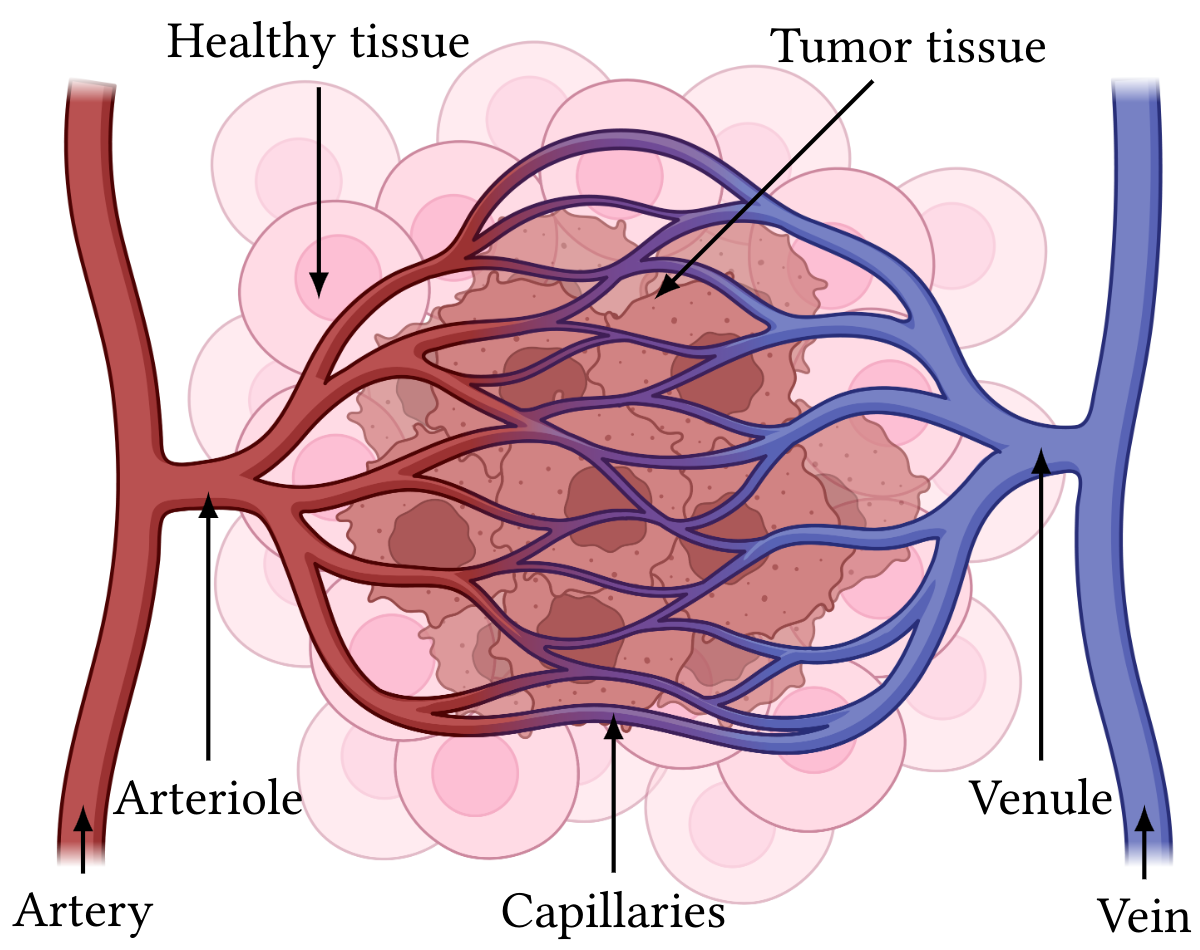
\includegraphics[angle=0,width=0.98\linewidth]{schematics.png}
	\vspace{1.0em}
}


%%% Bild 2 %%%%%%%%%%%%%%%%%%%%%%%%%%%%%%%%%%%%%%%%%%%%%%%%%%%%%%%%%%%%%%%%%%%%%
\headerbox{\textsf{Figure 2}}{name=bild2,column=3, span=2, below=bild1}{
	\centering
	\vspace{1.0em}
	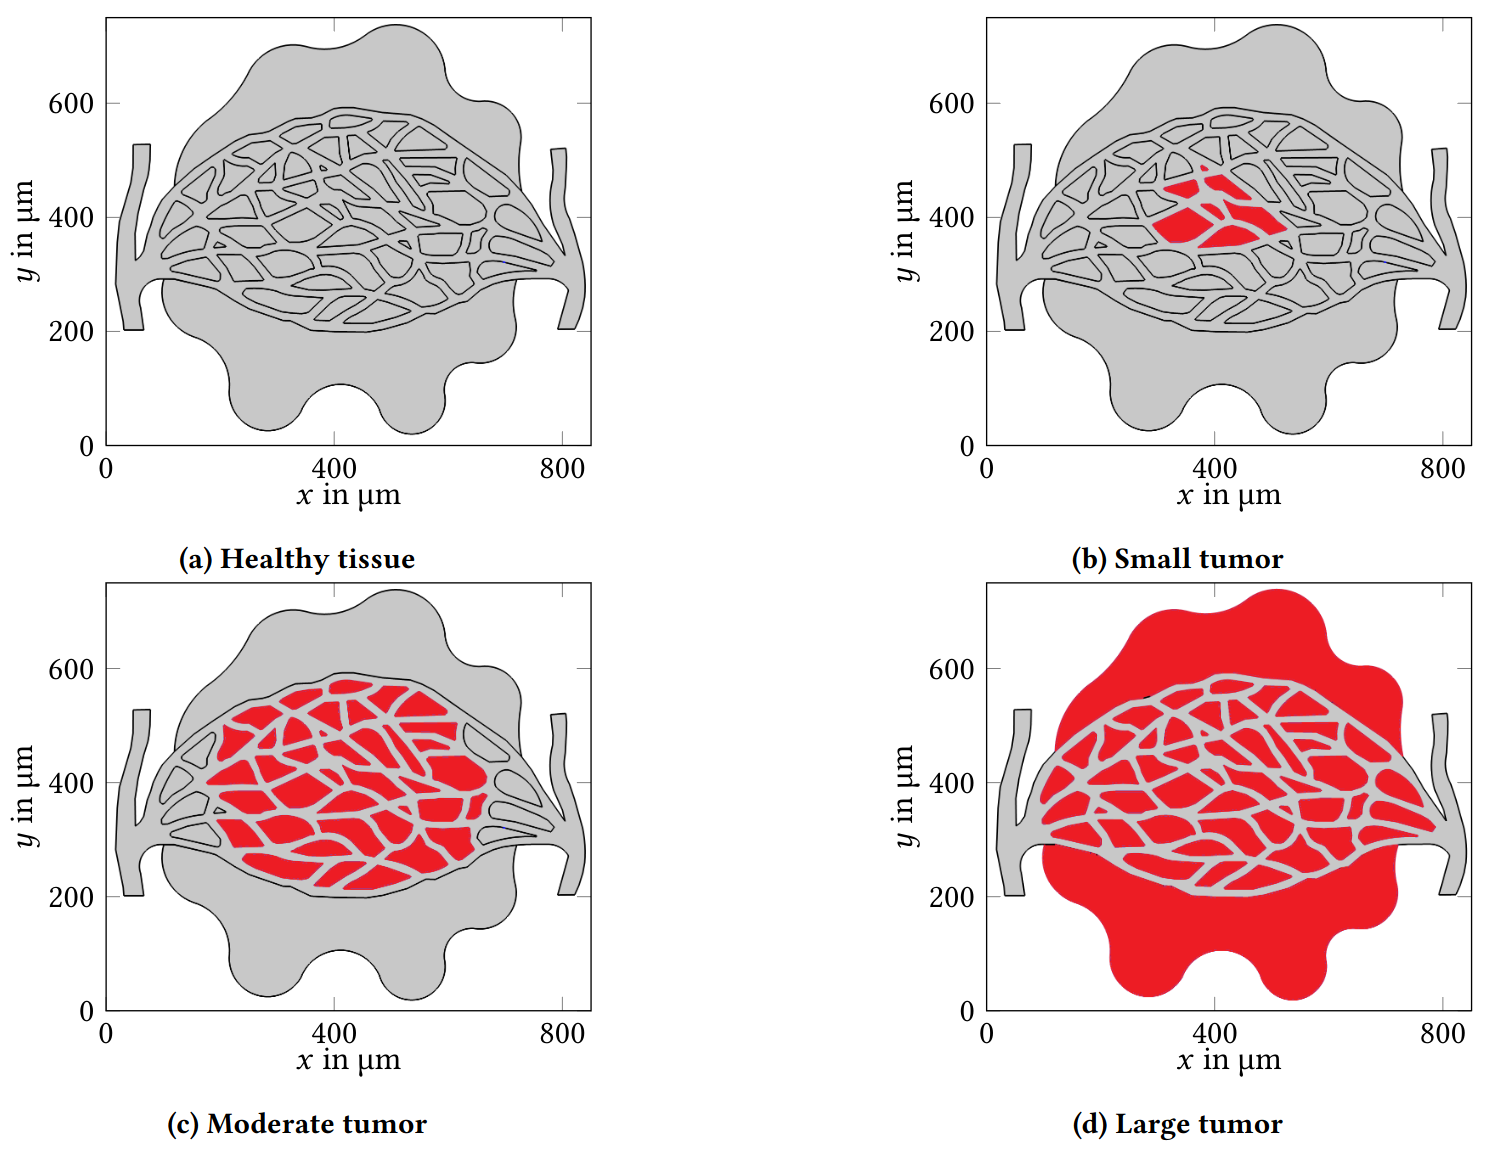
\includegraphics[angle=0,width=0.98\linewidth]{tumor_sizes.png}
	\vspace{1.0em}
}


%%% Bild 3 %%%%%%%%%%%%%%%%%%%%%%%%%%%%%%%%%%%%%%%%%%%%%%%%%%%%%%%%%%%%%%%%%%%%%
\headerbox{\textsf{Figure 3}}{name=bild3, column=3, span=2, below=bild2}{
	\centering
	\vspace{1.0em}
	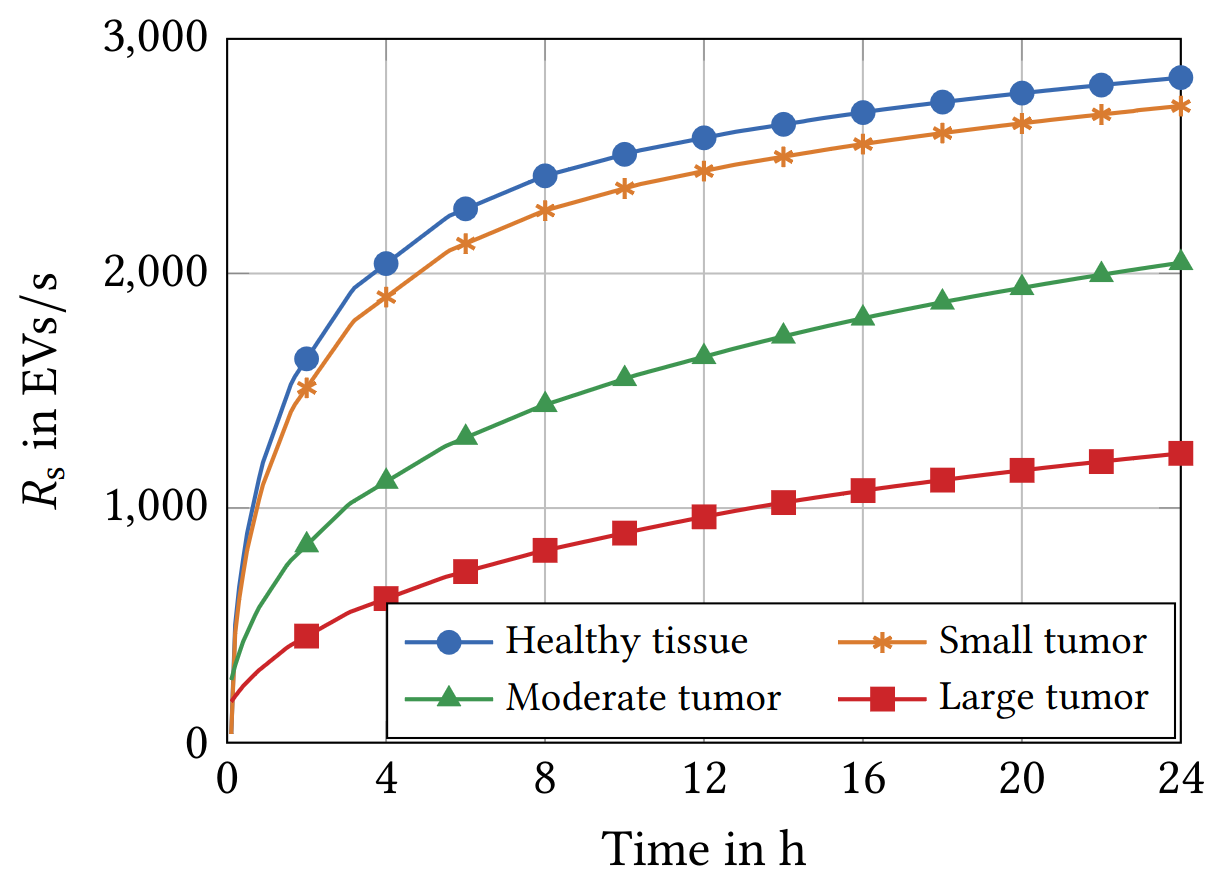
\includegraphics[angle=0,width=0.98\linewidth]{penetration_rate.png}
	\vspace{1.0em}
}

%%% References %%%%%%%%%%%%%%%%%%%%%%%%%%%%%%%%%%%%%%%%%%%%%%%%%%%%%%%%%%%%%%%%%%%%%
\headerbox{\textsf{Quellen}}{name=references, column=0, span=5, above=bottom, below=abschnitt4, below=bild3}{
%\smaller										% Make the whole text smaller
\vspace{1.0em} 								% Save some space at the beginning
\bibliographystyle{plain}						% Use plain style
\renewcommand{\section}[2]{\vskip 0.05em}		% Omit "References" title
\begin{thebibliography}{1}						% Simple bibliography with widest label of 1
\itemsep=-0.01em								% Save space between the separation
\setlength{\baselineskip}{0.4em}				% Save space with longer lines
\bibitem{prevWork1} Laszlo Gulyas, Richard Legendi: \emph{Effects of Sample Duration on Network Statistics in Elementary Models of Dynamic Networks}, International Conference on Computational Science, Singapore (2011) 
\end{thebibliography}
}

\end{poster}

\end{document}

